\documentclass[fleqn,10pt]{physiome}
% Use option lineno for line numbers

\articletype{Original}
%% Choose from Original, Retrospective, Review, Letter

\title{Example Article Title}

\author[1][corr.author@xyz.ac.mm]{First Author}
\author[2]{Second Author}
\affil[1]{Address of first author}
\affil[2]{Address of second author}

%% The following lines can be omitted when submitting;
%% information will be added by editors
\publicationdate{30 Sept 2020}
\editor{An Editor}
\curator{The Chief}
\submitteddate{4 May 2020}
\accepteddate{15 Sept 2020}
\citethisas{First and Second (2020) Example Article Title. Physiome 00(0).}{000.0000/a00000}
\begin{document}

\maketitle

\begin{abstract}
Please provide an abstract of no more than 300 words. Your abstract should explain the main contributions of your article, and should not contain any material that is not included in the main text.
\end{abstract}

\keywords{Keyword1, Keyword2, Keyword3}

\primarypubs[10.1037a0000000]{sample}{Aivazian917,Bloss029983}

\section{Introduction}

Your introduction goes here! Some examples of commonly used commands and features are listed below, to help you get started.

\section{Model description}

Guidelines can be included for standard research article sections, such as this one.

\subsection{Primary Publication}

Every \emph{Physiome} article needs to be associated with one or more Primary Publications. The Primary Publication is an experimental/modelling paper describing the model(s), that has been accepted to a peer-reviewed journal in the field of physiological modelling. The Primary Publication shows that the model is validated by describing the experiments and data, and the model(s) fit to the data, as well as the biological background and why the model is important.
\emph{Physiome} articles focus on reproducibility and reuse, but do not deal with the validation or scientific relevance of the models.

You can list the primary publications in a .bib file, then insert them after the \verb|\keywords{...}| using the \verb|\primepubs| command:

\verb|\primepubs{name of .bib file}{BibTeX keys of the publications}|

If your code is online, provide the link as an optional argument to \verb|\primepubs|:

\begin{verbatim}
    \primepubs[link to the model code]
      {name of .bib file}{BibTeX keys of the publications}|
\end{verbatim}

If you are authoring and compiling this template on your own machine, you will need to run an extra step \verb|bibtex primepub| to generate them in the final PDF. If you wish, you can use \texttt{latexmk}, \texttt{arara} or \texttt{Make} to automate this step.

\subsection{Some \LaTeX{} Examples}
\label{sec:examples}

Use section and subsection commands to organize your document. \LaTeX{} handles all the formatting and numbering automatically. Use \verb|\autoref| and \verb|\label| commands for cross-references, e.g.~\autoref{sec:examples}, \autoref{eq:sum}, \autoref{fig:view}, \autoref{tab:widgets}. You can still use the more common \verb|\ref|, but this will only generate the (sub)section/table/figure/equation number: \ref{tab:withnotes}.

\subsection{Figures and Tables}

Use the table and tabular commands for basic tables --- see \autoref{tab:widgets}, for example. \autoref{tab:withnotes} shows a larger example with \emph{table notes}. You can upload a figure (JPEG, PNG or PDF) using the project menu. To include it in your document, use the \verb|\includegraphics| command as in the code for \autoref{fig:view} below. Captions are always justified and start from the left; don't try to change the alignment.

If you prefer, you can place all your image files in a folder. Remember to include the folder path in your \verb|\includegraphics| command, or use `\verb|\graphicspath|` to specify the path to the folder in which all your image files can be found.

\begin{figure}[ht]\centering
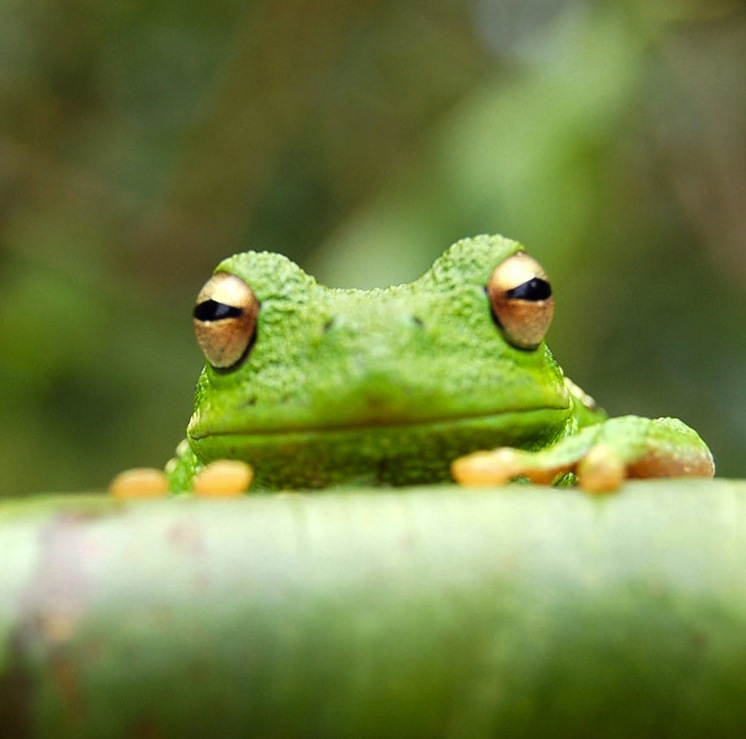
\includegraphics[width=0.5\linewidth]{frog}
\caption{An example image of a frog.}
\label{fig:view}
\end{figure}

\begin{table}[ht]\centering
\caption{An example table.}\label{tab:widgets}
\begin{tabular}{l r}
\toprule
Item & Quantity \\\midrule
Candles & 4 \\
Fork handles & ?\\
\bottomrule
\end{tabular}
\end{table}

\begin{table}[hbt!]\centering
\begin{threeparttable}
\caption{An example table with tablenotes}\label{tab:withnotes}

\begin{tabular}{lccrr}
\toprule
Variables & JKL ($n=30$) & Control ($n=40$) & MN & $t$ (68)\\
\midrule
Age at testing & 38 & 58\tnote{1} & 504.48 & 58 ms\\
Age at testing & 38 & 58 & 504.48 & 58 ms\\
Age at testing & 38 & 58 & 504.48 & 58 ms\\
Age at testing & 38 & 58 & 504.48 & 58 ms\\
Age at testing\tnote{2} & 38 & 58 & 504.48 & 58 ms\\
Age at testing & 38 & 58 & 504.48 & 58 ms\\
\bottomrule
\end{tabular}
\begin{tablenotes}
\item[1] JKL, just keep laughing.
\item[2] MN, merry noise.
\end{tablenotes}
\end{threeparttable}
\end{table}

\subsection{Citations}

LaTeX formats citations and references automatically using the bibliography records in your .bib file, which you can edit via the project menu. Use the \verb|\citet| command for a text citation, like \citet{lees2010theoretical}, and the \verb|\citep| command for a citation in parentheses \citep{McQuilton01012012}.

\subsection{Mathematics}

\LaTeX{} is great at typesetting mathematics. Let $X_1, X_2, \ldots, X_n$ be a sequence of independent and identically distributed random variables with $\text{E}[X_i] = \mu$ and $\text{Var}[X_i] = \sigma^2 < \infty$, and let
\begin{equation}\label{eq:sum}
S_n = \frac{X_1 + X_2 + \cdots + X_n}{n}
      = \frac{1}{n}\sum_{i}^{n} X_i
\end{equation}
denote their mean. Then as $n$ approaches infinity, the random variables $\sqrt{n}(S_n - \mu)$ converge in distribution to a normal $\mathcal{N}(0, \sigma^2)$.

\subsection{Lists}

You can make lists with automatic numbering \dots

\begin{enumerate}[noitemsep]
\item Like this,
\item and like this.
\end{enumerate}
\dots or bullet points \dots
\begin{itemize}[noitemsep]
\item Like this,
\item and like this.
\end{itemize}
\dots or with words and descriptions \dots
\begin{description}
\item[Word] Definition
\item[Concept] Explanation
\item[Idea] Text
\end{description}

\section{Model results}
Quam suscipit ut quidem et animi numquam consectetur et. Nihil et commodi ut officia eveniet beatae qui. Placeat accusantium eius consequatur animi nisi sed. Pariatur et dolores tempore velit similique voluptatem similique error.

Quam suscipit ut quidem et animi numquam consectetur et. Nihil et commodi ut officia eveniet beatae qui. Placeat accusantium eius consequatur animi nisi sed. Pariatur et dolores tempore velit similique voluptatem similique error. Quam suscipit ut quidem et animi numquam consectetur et. Nihil et commodi ut officia eveniet beatae qui. Placeat accusantium eius consequatur animi nisi sed. Pariatur et dolores tempore velit similique voluptatem similique error.

% \section{Discussion}

% Quam suscipit ut quidem et animi numquam consectetur et. Nihil et commodi ut officia eveniet beatae qui. Placeat accusantium eius consequatur animi nisi sed. Pariatur et dolores tempore velit similique voluptatem similique error.

% Quam suscipit ut quidem et animi numquam consectetur et. Nihil et commodi ut officia eveniet beatae qui. Placeat accusantium eius consequatur animi nisi sed. Pariatur et dolores tempore velit similique voluptatem similique error.

\bibliography{sample}

\end{document}
